\documentclass[11pt,letterpaper]{report}
%%%%%%%%%%%%%%%%%%%%%%%
%% Page layout
\usepackage{graphics,graphicx,wrapfig}
\usepackage[letterpaper, margin=2.5 cm, headheight=4 cm, top= 6cm]{geometry}
\setlength{\parindent}{0pt}
\usepackage{parskip}
\setlength{\parskip}{0.5em}

\usepackage{fancyhdr}
\usepackage{bm}
\usepackage{upgreek}

\fancyhf{}
\fancyhead[L]{

\includegraphics[height=3 cm]{Figures/Brown_Letterhead/H_2c_Pos}
\\
}
%
\fancyhead[C]{
\parbox[b][3.5cm][t]{4cm}{
\begin{flushright}
Haneesh Kesari
\\
Assistant Professor
\\
of Engineering
\\
\end{flushright}
}
}
%
\fancyhead[R]{
\parbox[b][3.5cm][t]{6cm}{
\begin{flushleft}
School of Engineering
\\
Brown University
\\
184 Hope Street, B\&H 612
\\
Providence, RI 02912
\\
Phone: 401-863-1418
\\
Email: Haneesh\_Kesari@brown.edu
\\
\end{flushleft}
}
}

\fancypagestyle{plain}{
\fancyhf{} % remove everything
%
\renewcommand{\headrulewidth}{0pt} % remove lines as well
%
\renewcommand{\footrulewidth}{0pt}
%
\fancyfoot[R]{\thepage / \pageref{LastPage}}
}
 
%% Fonts
\usepackage{amssymb,amsfonts,amsmath,amsthm}
\usepackage[T1]{fontenc}
\usepackage{mathptmx}
\usepackage{cmbright}
\usepackage{bm}

\usepackage{sectsty}
\sectionfont{\fontsize{16}{16}\selectfont}

%% typesetting
\usepackage{tabto}
\usepackage{upgreek}

%% colors
\usepackage[dvipsnames]{xcolor}
\definecolor{DarkRed}{rgb}{0.62, 0.16, 0.09}

%% referencing
\usepackage{nameref}
\usepackage{lastpage}
\usepackage[biblabel]{cite}
\usepackage[colorlinks=true,urlcolor=DarkRed,linkcolor=DarkRed,citecolor=black]{hyperref}

%% enumerate
\usepackage{enumerate}
\usepackage{enumitem}

%% floats
\usepackage{float}
\usepackage[font=footnotesize, labelfont={bf},labelsep=period]{caption}
\usepackage{booktabs}
\usepackage{threeparttable}

%% custom commands
\usepackage[scr=boondoxo]{mathalfa}
\newcommand{\loc}{\textit{LoC}}

\newcommand{\norm}[1]{\ensuremath \lVert #1 \rVert}

\newcommand{\ex}{{\bm{\hat{e}}}_1}
\newcommand{\ey}{{\bm{\hat{e}}}_2}
\newcommand{\ez}{{\bm{\hat{e}}}_3}
\newcommand{\ei}{{\bm{\hat{e}}}_i}
\newcommand{\ej}{{\bm{\hat{e}}}_j}
\newcommand{\er}{{\bm{\hat{e}}}_r}
\newcommand{\et}{{\bm{\hat{e}}}_\theta}
\newcommand{\ep}{{\bm{\hat{e}}}_\phi}

\usepackage{xspace}
\newcommand{\TA}{\textit{Ta.\@}\xspace}
\newcommand{\EA}{\textit{Ea.\@}\xspace}

%% checklist
\usepackage{enumitem,amssymb}
\newlist{todolist}{itemize}{2}
\setlist[todolist]{label=$\square$}
\usepackage{pifont}
\newcommand{\cmark}{\ding{51}}%
\newcommand{\xmark}{\ding{55}}%
\newcommand{\done}{\rlap{$\square$}{\raisebox{2pt}{\large\hspace{1pt}\cmark}}%
\hspace{-2.5pt}}
\newcommand{\wontfix}{\rlap{$\square$}{\large\hspace{1pt}\xmark}}


\renewcommand{\u}[1]{\boldsymbol{#1}}
\renewcommand{\t}[1]{\tilde{#1}}
\newcommand{\m}[1]{\mathbb{#1}}
\renewcommand{\c}[1]{\mathcal{#1}}
\newcommand{\lsc}[2][\mathscr{l}]{{}^{ #1 }\! #2}
\newcommand{\lscH}[1]{\lsc[H]{#1}}
\newcommand{\dsf}[1]{\Delta\boldsymbol{\sf #1}}
\newcommand{\tpsb}[1]{\left. #1 \right.^{\sf T}}
\newcommand{\tps}[1]{\left( #1 \right)^{\sf T}}
\newcommand{\usf}[1]{\boldsymbol{\sf #1}}
\newcommand{\busf}[1]{\bar{\usf{ #1}}}
\newcommand{\tu}[1]{\tilde{\u{ #1}}}
\newcommand{\tusf}[1]{\tilde{\usf{ #1}}}
\newcommand{\btusf}[1]{\bar{\tusf{ #1}}}
\newcommand{\pr}[1]{\left( #1 \right)}
\newcommand{\physe}{\hat{\mathbscr{e}}} %


\begin{document}

\newpage
\setcounter{page}{1}
%%%%%%%%%%%%%%%%%%%%%%%%%%%%%%%%%%%%%%%%%%%%%%%%%%%%%%
%%%%%%%%%%%%%%%%%%%%%%%%%%%%%%%%%%%%%%%%%%%%%%%%%%%%%%
%%%%%%%%%%%%%%%%%%%%%%%%%%%%%%%%%%%%%%%%%%%%%%%%%%%%%%
\thispagestyle{fancy}
\phantom{x}
\vspace{4em}
% \textbf{Author response letter to Reviewers}

Regarding: Point-by-point response to issues raised by referees  (manuscript JMBBM-D-21-00364).
%hk done

\vspace{3em}
Dear Editors and Reviewers,
%hk done
\vspace{1em}

We thank you for your very valuable feedback. In response to your feedback, we have made the revisions listed in the section \textit{List Of Changes} (\textit{LoC}), which can be found on  page \pageref{LoCpage} of this response letter. We  provide a point-by-point response to the Reviewers' comments in the following pages. Our responses to Reviewer \#1's and Reviewer \#2's comments can be found on pages \pageref{rev1} and \pageref{rev2}, respectively, of this response letter. Through these changes and our responses to your comments, we hope that we have addressed all of your concerns.

We thank you for your consideration of our revised manuscript.

\vspace{2em}
Sincerely,

Wenqiang Fang, Sayaka Kochiyama, and Haneesh Kesari

%%%%%%%%%%%%%%%%%%%%%%%%%%%%%%%%%%%%%%%%%%%%%%%%%%%%%%
%%%%%%%%%%%%%%%%%%%%%%%%%%%%%%%%%%%%%%%%%%%%%%%%%%%%%%
%%%%%%%%%%%%%%%%%%%%%%%%%%%%%%%%%%%%%%%%%%%%%%%%%%%%%%
\clearpage
\pagestyle{plain}
\newgeometry{margin=2.5 cm}
%%%%%%%%%%%%%%%%%%%%%%%%%%%%%%%%%%%%%%%%%%%%%%%%%%%%%%
\section*{List of Changes}
\label{LoCpage}

{\bf Changes in response to Reviewer criticisms}
% \begin{enumerate}[label=\textit{Mc.\arabic*}]
% %
% \item \label{a1} In response to Reviewer \#1's comment (listed as comment \ref{r1c3} of this letter) regarding the existing frameworks for estimating head accelerations, we have modified the third paragraph in page 4. We added the work of Genin \textit{et al.}~\cite{genin1997} as a reference.
% %
% \item \label{a2} In response to Reviewer \#1's comment (listed as comment \ref{r1c4} of this letter) regarding the existing frameworks for estimating head accelerations, we have modified the third paragraph in page 4. We added the works of Madgwick \textit{et al.}~\cite{madgwick2013} and Naunheim \textit{et al.}~\cite{naunheim2003} as references.
% \end{enumerate}

\clearpage
%%%%%%%%%%%%%%%%%%%%%%%%%%%%%%%%%%%%%%%%%%%%%%%%%%%%%%
\section*{Response to Reviewer \#1's comments}
\label{rev1}

\begin{enumerate}[label=\textit{1.\arabic*},wide, labelwidth=!, labelindent=0pt]

\item \label{r1c1} {\bf ``The authors have presented a good piece of work, through which they are able to explain the sawtooth patterns observed in the force-displacement curves. This is done by allowing for slippage at the test supports and paying attention to the coefficient of friction.''}

We thank the Reviewer for their consideration of our manuscript.

% \newpage
\item \label{r1c2} {\bf `` A few minor comments to help clarify and strengthen the work: a) In the SS experiments, how it is ascertained that the boundary conditions correspond to the simply supported conditions.''}

We thank the reviewer for the comments on helping clarify and strengthen the work.

In structural mechanics, the essential features of a simply supported condition are given as follows (see~\cite{gere1997mechanics}):
\begin{enumerate}[label=\textit{(SS\arabic*).},leftmargin = 1.5 cm]
\item The material points of the beam that are in contact with the supports cannot move vertically.
\item The material points of the beam that are in contact with the supports cannot develop a moment reaction.
\end{enumerate}


As for the setup in our SS experiments, we provided a schematic of the simply-supported setup in Fig. 5 of the submitted manuscript, in which the spicule is suspended over a trench. This suggests that SS1 is guaranteed. Photos of the experimental setup and the mechanical testing device can be found in Fig. 5 of~\cite{kochiyama2021sawtooth} and Fig. 2 of~\cite{monn2017enhanced}, respectively. From the photos, we clearly see the spicules' segments beyond the trench edges are straight, which suggests that SS2 is valid. 

Furthermore, we applied Euler-Bernoulli (EB) theory with simply-supported boundary condition to the SS experiments of spicules. From the experimentally measured force-deflection curves, we computed the Young's modulus of the tested spicules. For given applied forces, we were able to predict the deformed shapes of the spicules using EB theory with the calculated Young's modulus. When comparing the predictions with the optical micrographs of the spicules' deformed shapes, we found they match each other extremely well (for example, see Fig. 4(D) of~\cite{monn2017enhanced}). Therefore, we are certain that the boundary conditions in the SS experiments correspond to the simply supported conditions.


% \newpage
\item \label{r1c3} {\bf ``b) The experiments all appear to be conducted for a static loading and this needs to be pointed out explicitly, in particular, when using friction in the model. The time scales over which the loading could be critical if dynamic friction is involved. Can any relevant details be provided in the paper?
''}


% ``The loading phase of the tests were conducted by moving the MTS in
% the~$-\physe_2$ direction at a rate of~$1~\mu$m/sec.'' in the last paragraph in page 9 of the manuscript.

\item \label{r1c4} {\bf ``
c) With regard to the elastica theory, an extension would be the rod theory, which would be needed for a three-dimensional setting; see Antman, S. S., Problems in Nonlinear Elasticity, Springer.''}

Although we have introduced our mathematical notions and definitions in a general three-dimensional context, we clearly stated that our modelling the spicule's deformation is two dimensional in the last paragraph in page 6 of the manuscript:
``Considering the geometry in the SS experiments (e.g., see Figure~2), in our model we take that the spicule's displacements to be two dimensional in nature.'' 

We were looking for an extension of Euler-Bernoulli (EB) theory to the regime of large displacements and rotations in our study. We believe Euler's elastica theory is sufficient and mathematically tractable. 
The rod theory is a more general extension of elastica theory, which accounts for not only flexure, but also extension and shear. 
In our experimental setup, the effects of extension and shear do not play an important role in the deformation of the spicules. Thus we believe that it is reasonable to ignore the effects of extension and shear in the model. Therefore, we modeled the spicules' deformation using Euler's elastica theory. 


% \begin{figure}
% \centering{}
% 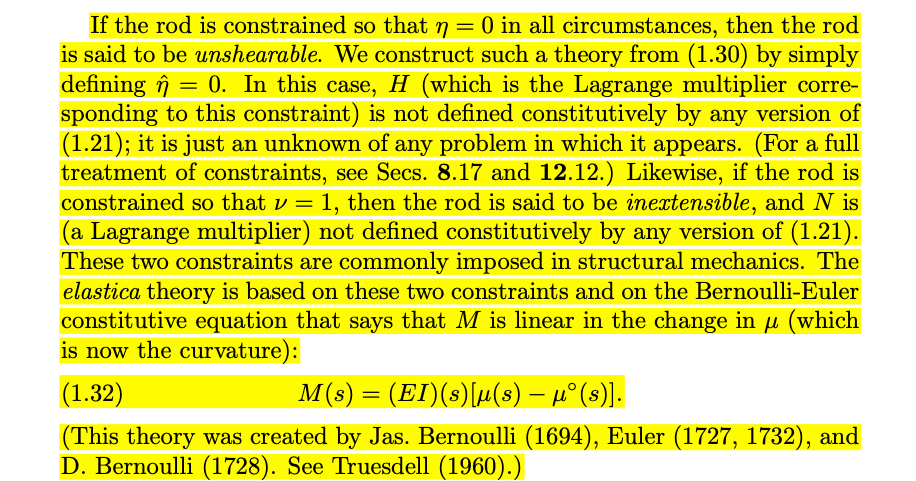
\includegraphics[width = 1.0\textwidth]{Figures/Antman.png}
% \end{figure}
% \end{enumerate}


\clearpage

%%%%%%%%%%%%%%%%%%%%%%%%%%%%%%%%%%%%%%%%%%%%%%%%%%%%%%
\section*{Response to Reviewer \#2's comments}
\label{rev2}

\begin{enumerate}[label=\textit{2.\arabic*},wide, labelindent=0pt]

\item \label{r2c1}{\bf ``The authors report on the three-point bending tests of marine sponge fibers and the possible mechanism for the sawtooth-pattern during the bending tests. They argued that the sawtooth-pattern is originated from the stick-slip motion on the supporting substance and eliminated the Cook-Gordon mechanism. 
While Cook-Gordon mechanism is valid during the fracture of the materials, I am curious whether the experiment here caused the fracture of the spicule? 
If not, then the bending of spicule may remain in the "elastic deformation" and the stick-slip should be caused by the friction on the supporting layer, as stated by the authors. Then the initial argument is meaningless. 
If yes, how is the fractured surface looks like? Will the propagation of cracks have any correlation to the sawtooth-pattern? ''}


We have reported three-point bending tests on many different marine sponge spicules that display sawtooth patterns in our manuscript. All experiments using simply-supported setup have caused the fracture of the spicules.
Optical images of the fractured surfaces are shown in Fig. 4(B) and (C) of~\cite{kochiyama2021sawtooth} for \textit{Monorhaphis chuni} anchor spicules and \textit{Rosella racovitzae} spicules, and Fig. 3(G) of~\cite{monn2017enhanced} for \textit{Euplectella aspergillum} (\textit{Ea.}) anchor spicules. 
Although we only tested \textit{Ea.} spicules on our own, we brought up \textit{M. chuni} and \textit{R. racovitzae} in order to argue that our hypothesis and model can be applied to a broader range of structural biological materials. 

In order to get direct evidence of whether the propagation of cracks have any correlation to the sawtooth patterns, it is necessary to monitor the crack propagation constantly during the three-point bending test. However, as the crack may grow inside the spicules, optical micrographs can not provide such evidence. Sophisticated experimental design involving electric circuit may be effective for the purpose of monitoring crack propagation.
Since we have difficulty monitoring the crack propagation during our tests, we cannot conclude whether the propagation of cracks have any correlation to the sawtooth pattern solely from the final fractured surfaces of the spicules after the tests. 



\item \label{r2c2}{\bf ``The labelling of figures is chaos! The language should be polished, it is quite spoken language.''}
\end{enumerate}

In response to the reviewer's above comments, we have made modifications to the labeling of Fig. 3 and revised the language of some of the sentences in the manuscripts. 


\end{enumerate}

\clearpage

%%%%%%%%%%%%%%%%%%%%%%%%%%%%%%%%%%%%%%%%%%%%%%%%%%%%%%
\bibliographystyle{apalike}
\bibliography{refs}

\end{document}
